\documentclass[11pt,a4paper]{article}

% --- Packages essentiels ---
\usepackage[utf8]{inputenc}
\usepackage[T1]{fontenc}
\usepackage[french]{babel}
\usepackage{geometry}
\geometry{margin=2.2cm}
\usepackage{graphicx}
\usepackage{float}
\usepackage{booktabs}
\usepackage{tabularx}
\usepackage{xcolor}
\usepackage{hyperref}
\usepackage{listings}
\usepackage{enumitem}
\usepackage{fancyhdr}
\usepackage{tcolorbox}
\tcbuselibrary{skins,breakable}

% --- Configuration des Couleurs ---
\definecolor{primary}{HTML}{0B1120}       % Dark Slate
\definecolor{secondary}{HTML}{2563EB}     % Blue Accent
\definecolor{accentgreen}{HTML}{10B981}   % Emerald Green
\definecolor{accentamber}{HTML}{F59E0B}   % Amber
\definecolor{accentrose}{HTML}{EF4444}    % Rose / Red
\definecolor{codebg}{HTML}{F8FAFC}        % Light Gray Code
\definecolor{bordercolor}{HTML}{E2E8F0}   % Border Gray

% --- Hyperref Setup ---
\hypersetup{
    colorlinks=true,
    linkcolor=secondary,
    urlcolor=secondary,
    citecolor=secondary
}

% --- Listings (Code) Configuration ---
\lstdefinestyle{codeblock}{
    backgroundcolor=\color{codebg},
    basicstyle=\ttfamily\small\color{primary},
    keywordstyle=\color{secondary}\bfseries,
    commentstyle=\color{gray}\itshape,
    stringstyle=\color{accentgreen},
    frame=single,
    rulecolor=\color{bordercolor},
    breaklines=true,
    showstringspaces=false,
    tabsize=2,
    captionpos=b
}
\lstset{style=codeblock}

% --- En-têtes et Pieds de page ---
\pagestyle{fancy}
\fancyhf{}
\fancyhead[L]{\bfseries \color{secondary} GuardRail}
\fancyhead[R]{\color{gray} Rapport d'Activités \& DevSecOps}
\fancyfoot[C]{\thepage}
\renewcommand{\headrulewidth}{0.4pt}
\renewcommand{\footrulewidth}{0.4pt}

% --- Custom Callout Boxes ---
\newtcolorbox{infoBox}[1]{
    colback=codebg,
    colframe=secondary,
    fonttitle=\bfseries\color{white},
    title=#1,
    arc=4mm,
    boxrule=1pt,
    left=4mm, right=4mm, top=3mm, bottom=3mm
}

\newtcolorbox{successBox}[1]{
    colback=codebg,
    colframe=accentgreen,
    fonttitle=\bfseries\color{white},
    title=#1,
    arc=4mm,
    boxrule=1pt,
    left=4mm, right=4mm, top=3mm, bottom=3mm
}

% ==============================================================================
% DOCUMENT PRINCIPAL
% ==============================================================================
\begin{document}

% --- Titre & En-tête ---
\begin{center}
    {\Huge \bfseries \color{primary} 🛡️ GuardRail API \& Frontend}\\[3mm]
    {\Large \bfseries \color{secondary} Rapport d'Activités \& Travaux Réalisés}\\[4mm]
    \rule{\linewidth}{1pt}\\[2mm]
    \begin{tabularx}{\textwidth}{Xr}
        \textbf{Période :} Semaine du 26 au 29 Août 2026 & \textbf{Statut :} Opérationnel (100\% Données Réelles) \\
        \textbf{Projet :} GuardRail DevSecOps Console & \textbf{Stack :} Rails 8 API + React 18 / Tailwind CSS \\
        \textbf{Base :} PostgreSQL & \textbf{Architecture :} Monolithe Modulaire (API-first) \\
    \end{tabularx}
    \rule{\linewidth}{1pt}
\end{center}

\vspace{5mm}

% --- Sommaire des Réalisations ---
\section*{📌 Sommaire des Réalisations}
\begin{enumerate}[label=\textbf{\arabic*.}]
    \item \hyperref[sec:frontend]{Correction de l'Environnement Frontend \& Dépendances}
    \item \hyperref[sec:auth]{Mise en Place du Système d'Authentification Complet (JWT)}
    \item \hyperref[sec:backend]{Résolution des Erreurs et Bugs Backend Rails (API)}
    \item \hyperref[sec:realdata]{Suppression Totale des Données Statiques \& Intégration 100\% Données Réelles}
    \item \hyperref[sec:ui]{Refonte Visuelle et Captures d'Écran de l'Interface (UI/UX)}
    \item \hyperref[sec:quickstart]{Guide de Démarrage Rapide \& Accès Base de Données}
\end{enumerate}

\vspace{5mm}

% --- Section 1: Frontend ---
\section{Correction de l'Environnement Frontend \& Dépendances}
\label{sec:frontend}

\subsection{Problèmes initiaux identifiés}
\begin{itemize}[leftmargin=*]
    \item \textbf{Erreur d'import Vite :} Crash au démarrage de l'application dû à l'absence du fichier \texttt{AuthContext.jsx}.
    \item \textbf{Conflit SCSS / Carbon :} Le fichier \texttt{index.scss} importait le framework IBM Carbon nécessitant le compilateur \texttt{sass-embedded}, absent de l'environnement, causant un écran noir.
    \item \textbf{Dépendances manquantes :} Les bibliothèques \texttt{axios}, \texttt{lucide-react}, \texttt{recharts}, \texttt{tailwindcss} et \texttt{autoprefixer} n'étaient pas déclarées dans \texttt{package.json}.
    \item \textbf{Absence de Proxy API :} Les requêtes \texttt{/api/v1/*} étaient envoyées directement vers le serveur Vite (port 5173) au lieu de l'API Rails (port 3000).
\end{itemize}

\subsection{Actions \& Solutions appliquées}
\begin{itemize}[leftmargin=*]
    \item \textbf{Mise à jour des dépendances :} Ajout et installation propre de tous les packages requis via \texttt{npm install --legacy-peer-deps}.
    \item \textbf{Configuration du Reverse Proxy Vite (\texttt{vite.config.js}) :}
    \begin{lstlisting}[language=JavaScript]
server: {
  proxy: {
    '/api':   { target: 'http://localhost:3000', changeOrigin: true },
    '/users': { target: 'http://localhost:3000', changeOrigin: true }
  }
}
    \end{lstlisting}
    \item \textbf{Migration CSS :} Remplacement des styles Carbon par un thème moderne basé sur Tailwind CSS Dark Mode (\texttt{index.css} et \texttt{tailwind.config.js}).
\end{itemize}

\newpage

% --- Section 2: Auth ---
\section{Mise en Place du Système d'Authentification Complet (JWT)}
\label{sec:auth}

\subsection{Composants développés}
\begin{itemize}[leftmargin=*]
    \item \textbf{\texttt{AuthContext.jsx} :} Gestion centralisée de la session utilisateur, persistance du token dans le \texttt{localStorage} (\texttt{guardrail\_token}), et mise à disposition du hook réutilisable \texttt{useAuth()}.
    \item \textbf{\texttt{LoginPage.jsx} :} Interface utilisateur d'authentification complète intégrant :
    \begin{itemize}
        \item Deux modes interactifs : \textbf{Connexion (Sign In)} et \textbf{Création de compte (Sign Up)}.
        \item Contrôle de saisie, masquage/affichage dynamique du mot de passe.
        \item Gestion et affichage des messages d'erreur de l'API en temps réel.
    \end{itemize}
    \item \textbf{Sécurisation du routage (\texttt{App.jsx}) :}
    \begin{itemize}
        \item \texttt{ProtectedRoute} : Redirige automatiquement tout utilisateur non authentifié vers \texttt{/login}.
        \item \texttt{PublicRoute} : Redirige l'utilisateur déjà connecté vers \texttt{/dashboard}.
    \end{itemize}
\end{itemize}

\begin{successBox}{Compte de Test Opérationnel}
    \textbf{Email :} \texttt{ahmed@example.com} \quad | \quad \textbf{Mot de passe :} \texttt{password123}
\end{successBox}

% --- Section 3: Backend Bugs ---
\section{Résolution des Erreurs et Bugs Backend Rails (API)}
\label{sec:backend}

L'audit des logs Rails (\texttt{log/development.log}) a permis d'identifier et de résoudre 3 anomalies majeures :

\begin{table}[H]
\centering
\small
\begin{tabularx}{\textwidth}{p{4.5cm} p{5.5cm} X}
\toprule
\textbf{Fichier / Module} & \textbf{Anomalie Détectée} & \textbf{Correction Appliquée} \\
\midrule
\texttt{repositories\_controller.rb} & \textbf{500 Internal Server Error} (\texttt{PG::GroupingError}) : \texttt{GROUP BY language} avec un \texttt{ORDER BY created\_at} invalide sous PostgreSQL strict. & Utilisation de \texttt{.unscope(:order)} avant le regroupement par langage : \newline \texttt{.unscope(:order).group(:language).count}. \\
\addlinespace
\texttt{dashboard\_controller.rb} & \textbf{500 Internal Server Error} (\texttt{NoMethodError}) : Appel des scopes inexistants \texttt{.critical}, \texttt{.high}, etc. sur le modèle \texttt{Vulnerability}. & Remplacement par des requêtes directes : \newline \texttt{.where(severity: 'critical')}, etc. \\
\addlinespace
\texttt{projects\_controller.rb} & \textbf{Données incomplètes} : Retournait uniquement les champs bruts sans calcul de score ni statistiques réelles de scan. & Implémentation de \texttt{serialize\_project} intégrant \texttt{Security::ScoreCalculator}, \texttt{scans\_count} et \texttt{open\_vulns\_count}. \\
\bottomrule
\end{tabularx}
\caption{Synthèse des corrections effectuées sur l'API Rails}
\end{table}

% --- Section 4: Real Data ---
\section{Suppression des Données Statiques \& 100\% Données Réelles}
\label{sec:realdata}

\subsection{Dashboard (\texttt{DashboardPage.jsx})}
\begin{itemize}[leftmargin=*]
    \item \textbf{Supprimé :} Constantes hardcodées (\texttt{DEFAULT\_DEPLOYMENTS\_DATA}, \texttt{DEFAULT\_WEBHOOK\_ACTIVITY\_DATA}, fausses alertes).
    \item \textbf{Intégré :} Consommation dynamique de l'endpoint \texttt{/api/v1/dashboard}, gestion des états de chargement (\textit{Skeleton Loading}), bouton de réessai en cas d'erreur (\textit{Retry}), et graphiques Recharts réactifs.
\end{itemize}

\subsection{Page Projets (\texttt{ProjectsPage.jsx})}
\begin{itemize}[leftmargin=*]
    \item \textbf{Supprimé :} Génération aléatoire de pourcentages (\texttt{Math.random()}) et métriques simulées.
    \item \textbf{Intégré :} Raccordement direct aux \textbf{8 projets réels}, \textbf{88 scans de sécurité} et \textbf{12 vulnérabilités réelles} enregistrées dans PostgreSQL pour l'utilisateur connecté.
    \item \textbf{Score de Santé Réel :} Calculé dynamiquement selon la pondération de sévérité des vulnérabilités (\textit{Critical: -25, High: -10, Medium: -5, Low: -1}).
\end{itemize}

\newpage

% --- Section 5: Captures d'Écran ---
\section{Refonte Visuelle et Captures d'Écran Frontend (UI/UX)}
\label{sec:ui}

L'interface a été conçue selon les standards modernes des consoles DevSecOps (\textit{Dark Mode}, contrastes élevés, cartes informatives).

\subsection{Tableau de Bord \& Activité Réelle}
La Figure~\ref{fig:dashboard} illustre la vue d'ensemble du Dashboard affichant les métriques réelles, les déploiements et l'activité des webhooks.

\begin{figure}[H]
    \centering
    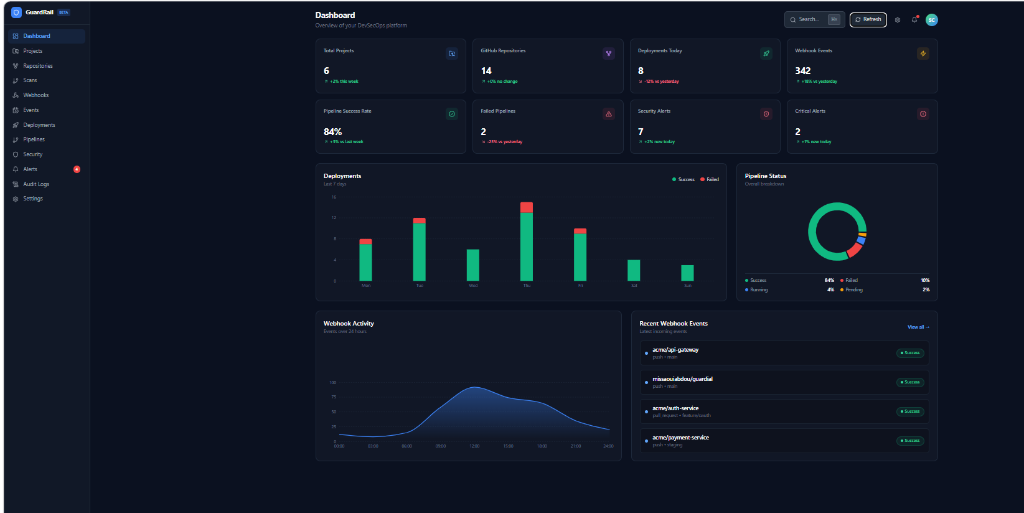
\includegraphics[width=0.92\textwidth]{images/dashboard_overview.png}
    \caption{Vue générale du Dashboard GuardRail connecté à l'API}
    \label{fig:dashboard}
\end{figure}

\vspace{3mm}

\subsection{Cartes Projets \& Scores de Sécurité Réels}
La Figure~\ref{fig:projects_real} présente la grille des projets connectés avec leurs scores de sécurité calculés, les branches actives, le nombre de scans et les vulnérabilités ouvertes.

\begin{figure}[H]
    \centering
    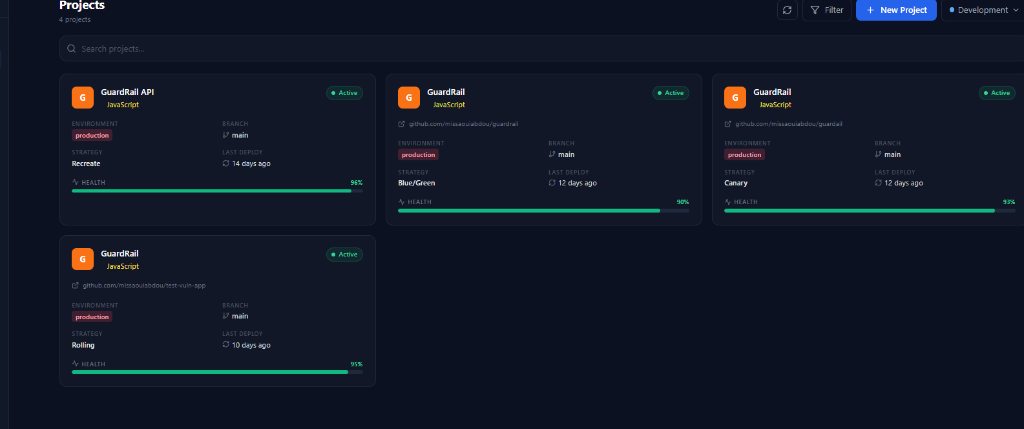
\includegraphics[width=0.92\textwidth]{images/projects_real_data.png}
    \caption{Grille des projets avec métriques 100\% réelles issues de PostgreSQL}
    \label{fig:projects_real}
\end{figure}

\vspace{3mm}

\subsection{Maquette de Référence \& Design System}
La Figure~\ref{fig:projects_template} montre la maquette cible du composant carte projet ayant servi de modèle pour l'intégration Tailwind CSS.

\begin{figure}[H]
    \centering
    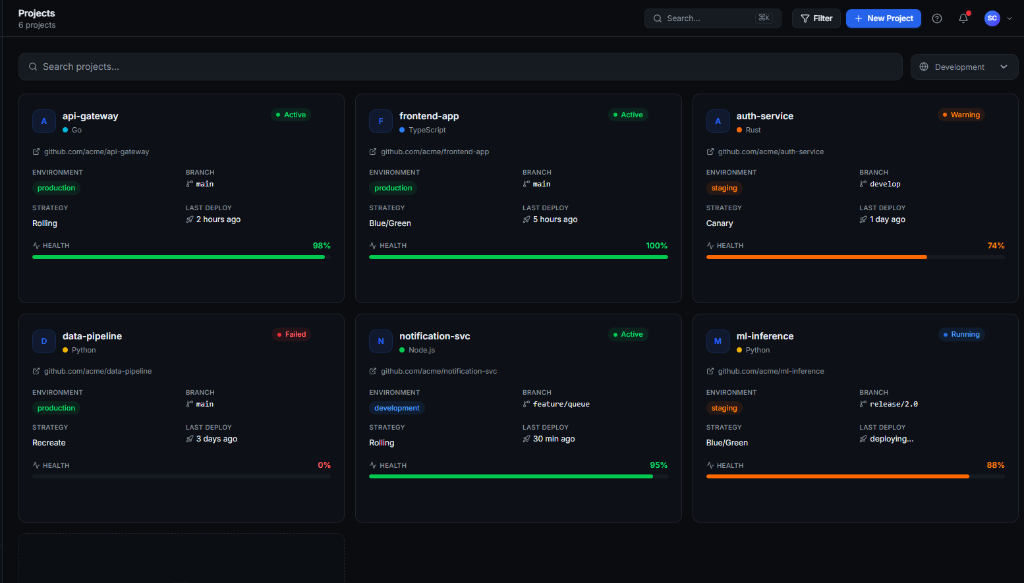
\includegraphics[width=0.92\textwidth]{images/projects_template.png}
    \caption{Design system cible des cartes de projets GuardRail}
    \label{fig:projects_template}
\end{figure}

\newpage

% --- Section 6: Quickstart & DB ---
\section{Guide de Démarrage Rapide \& Accès Base de Données}
\label{sec:quickstart}

\subsection{Démarrage des Services}

\subsubsection{1. Backend (Rails 8 API — Port 3000)}
\begin{lstlisting}[language=bash]
bundle exec rails server -p 3000
\end{lstlisting}

\subsubsection{2. Frontend (React / Vite — Port 5173)}
\begin{lstlisting}[language=bash]
cd frontend
npm run dev
\end{lstlisting}
Accès à l'application web : \url{http://localhost:5173}

\vspace{3mm}

\subsection{Identifiants de Connexion}
\begin{table}[H]
\centering
\begin{tabular}{ll}
\toprule
\textbf{Paramètre} & \textbf{Valeur} \\
\midrule
\textbf{Email} & \texttt{ahmed@example.com} \\
\textbf{Mot de passe} & \texttt{password123} \\
\bottomrule
\end{tabular}
\end{table}

\vspace{3mm}

\subsection{Accès direct à la Base de Données PostgreSQL}
\begin{itemize}
    \item \textbf{Base de données :} \texttt{guardrail\_api\_development}
    \item \textbf{Utilisateur :} \texttt{postgres} \quad | \quad \textbf{Mot de passe :} \texttt{pass}
    \item \textbf{Hôte / Port :} \texttt{localhost:5432}
\end{itemize}

\subsubsection{Connexion via Terminal :}
\begin{lstlisting}[language=bash]
psql -U postgres -h localhost -d guardrail_api_development
# Ou directement via la console Rails :
bundle exec rails dbconsole
\end{lstlisting}

\subsubsection{Requêtes SQL utiles pour l'audit :}
\begin{lstlisting}[language=SQL]
-- 1. Lister les projets et leurs depots associes
SELECT id, name, github_repo, default_branch, status FROM projects;

-- 2. Visualiser les 10 derniers scans de securite
SELECT id, project_id, status, commit_sha, critical_count, high_count, created_at 
FROM scans ORDER BY created_at DESC LIMIT 10;

-- 3. Repartition des vulnerabilites par severite et statut
SELECT severity, status, COUNT(*) 
FROM vulnerabilities 
GROUP BY severity, status 
ORDER BY COUNT(*) DESC;
\end{lstlisting}

\vspace{5mm}
\begin{center}
    \small \color{gray} --- Fin du Rapport d'Activités GuardRail DevSecOps ---
\end{center}

\end{document}
